\documentclass[letterpaper, 12pt]{math}

\usepackage{amsmath}
\usepackage{tikz}

\title{Multivariable and Vector Calculus}
\author{Alvin Lin}
\date{August 2017 - December 2017}

\begin{document}

\maketitle

\section*{Vectors}
\[ A(a_{1},a_{2},a_{3}) \]
\[ B(b_{1},b_{2},b_{3}) \]
\[ \vec{AB} = \langle b_{1}-a_{1},b_{2}-a_{2},b_{3}-a_{3}\rangle \]

\subsection*{Vector Operations}
\[ \vec{a}+\vec{b} = \langle a_{1}+b_{1},a_{2}+b_{2},a_{3}+b_{3}\rangle \]
\[ \lambda\vec{a} = \langle\lambda a_{1},\lambda a_{2},\lambda a_{3}\rangle \]
\[ |\vec{a}| = \sqrt{a_{1}^{2}+a_{2}^{2}+a_{3}^{2}} \]
\[ |\lambda\vec{a}| = |\lambda||\vec{a}| \]
\[ \lambda(\vec{a}+\vec{b}) = \lambda\vec{a}+\lambda\vec{b} \]
\[ \vec{a} = \langle a_{1},a_{2},a_{3}\rangle =
  |\vec{a}|\langle\frac{a_{1}}{|\vec{a}|}\frac{a_{2}}{|\vec{a}|}
  \frac{a_{3}}{|\vec{a}|}\rangle =
  |\vec{a}|\langle\cos(\alpha),\cos(\beta),\cos(\gamma)\rangle \]

\subsubsection*{Example}
Draw \( 2\vec{a}-\frac{1}{3}\vec{b} \):
\begin{center}
  \begin{tikzpicture}[scale=0.8]
    \node (O) at (0,0) {O};
    \node (A) at (2,2) {\( \vec{a} \)};
    \node (2A) at (4,4) {\( 2\vec{a} \)};
    \node (B) at (6,-3) {\( \vec{b} \)};
    \node (13B) at (-2,1) {\( \frac{1}{3}B \)};
    \node (SUM) at (2,5) {\( 2\vec{a}-\frac{1}{3}\vec{b} \)};
    \draw[->] (O) edge (B);
    \draw[->] (O) edge (A);
    \draw[->] (O) edge (2A);
    \draw[->] (O) edge (13B);
    \draw[->] (O) edge (SUM);
  \end{tikzpicture}
\end{center}

\subsubsection*{Example}
Given the vector of length 7 which makes an angle of \( 15^{\circ} \) with
\( \langle3,3\rangle \).
\[ \vec{a} = 7\langle\cos(30),\cos(60)\rangle =
  7\langle\frac{\sqrt{3}}{2},\frac{1}{2}\rangle =
  \langle\frac{7\sqrt{3}}{2},\frac{7}{2}\rangle \]
Alternate Solution:
\[ \vec{a} = 7\langle\cos(60),\cos(30)\rangle =
  7\langle\frac{1}{2},\frac{\sqrt{3}}{2}\rangle =
  \langle\frac{7}{2},\frac{7\sqrt{3}}{2}\rangle \]

\subsubsection*{Example}
A pilot steers a plane at 500mph towards N 30 E, while the wind blows at 200mph
from N 45 W. Find the true course and speed.
\begin{align*}
  \vec{t} &= \overrightarrow{pilot}+\overrightarrow{wind} \\
  &= 500\langle\cos(60),\cos(30)\rangle+200\langle\cos(45),-\cos(45)\rangle \\
  &= \langle250,250\sqrt{3}\rangle+\langle100\sqrt{2},-100\sqrt{2}\rangle \\
  &= \langle250+100\sqrt{2},250\sqrt{3}-100\sqrt{2}\rangle
\end{align*}

\subsubsection*{Example}
Give a vector of length 3, tangent to \( y = 2\sin(x) \) at
\( \frac{\pi}{6},1 \).
\begin{align*}
  y' &= 2\cos(x) \\
  y'(\frac{\pi}{6}) = \sqrt{3} \\
  \vec{v} &= \langle1,\sqrt{3}\rangle \\
  |\vec{v}| &= 2 \\
  \frac{3\vec{v}}{|\vec{v}|} &= \langle\frac{3}{2},\frac{\sqrt{3}}{2}\rangle
\end{align*}

\subsection*{Dot/scalar Product}
\[ \vec{a}\cdot\vec{b} = a_{1}b_{1}+a_{2}b_{2}+a_{b}b_{3} =
   \sum_{i}^{n}a_{i}b_{i} \]
Properties:
\begin{align*}
  \vec{a}\cdot\vec{a} &= |\vec{a}|^{2} \\
  \vec{a}\cdot\vec{b} &= \vec{b}\cdot\vec{a} \\
  \vec{a}\cdot(\vec{b}+\vec{c}) &= \vec{a}\cdot\vec{b}+\vec{a}\cdot\vec{c} \\
  (\lambda\vec{a})\cdot\vec{b} &= \lambda(\vec{a}\cdot\vec{b}) \\
  \vec{a}\cdot\vec{b} &= 0 \quad (\vec{a}\bot\vec{b})
\end{align*}
Law of Cosines:
\begin{center}
  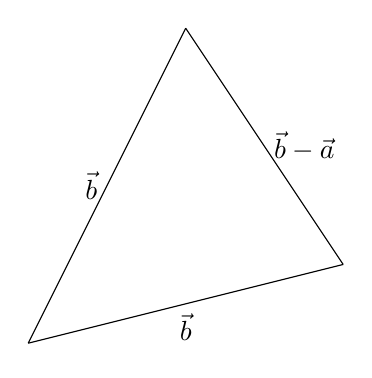
\begin{tikzpicture}
    \draw (0,0)--(4,1) node[pos=0.5, below] {\( \vec{b} \)};
    \draw (4,1)--(2,4) node[pos=0.5, right] {\( \vec{b}-\vec{a} \)};
    \draw (2,4)--(0,0) node[pos=0.5, left] {\( \vec{b} \)};
  \end{tikzpicture}
\end{center}
\[ |\vec{a}-\vec{b}|^{2} = |\vec{a}|^{2}+|\vec{b}|^{2}-
  2|\vec{a}||\vec{b}|\cos(\theta) \]
Using the vector properties:
\begin{align*}
  (\vec{b}-\vec{a})\cdot(\vec{b}-\vec{a}) &=
    \vec{a}\cdot\vec{a}+\vec{b}\cdot\vec{b}-2|\vec{a}||\vec{b}|\cos\theta \\
  \vec{a}\cdot\vec{b} &= |\vec{a}||\vec{b}|\cos\theta
\end{align*}

\subsubsection*{Example}
\[ \vec{a} = \langle1,2,3\rangle, \vec{b} = \langle2,x,4\rangle \]
For what x is \( \vec{a}\bot\vec{b} \):
\begin{align*}
  \vec{a}\cdot\vec{b} &= \langle1,2,3\rangle\cdot\langle2,x,4\rangle \\
  &= 2+2x+12 = 0 \\
  2x &= -14 \\
  x &= -7
\end{align*}

\subsubsection*{Example}
Given a triangle ABC where A(1,1,2), B(2,4,3), C(3,5,8), find angle
\( \angle CAB \). Let \( \alpha = \angle CAB \).
\begin{align*}
  \cos\alpha &= \frac{\overrightarrow{AB}\cdot\overrightarrow{AC}}
  {|\overrightarrow{AB}||\overrightarrow{AC}|} \\
  &= \frac{\langle1,3,1\rangle\cdot\langle2,4,6\rangle}
    {|\langle1,3,1\rangle||\langle2,4,6\rangle|} \\
  &= \frac{2+12+6}{\sqrt{11}\sqrt{56}} \\
  &= \frac{20}{\sqrt{11}\sqrt{56}} \\
  \alpha &= \arccos(\frac{20}{\sqrt{11}\sqrt{56}})
\end{align*}

\subsubsection*{Example}
Given two lines:
\[ l_{1}: x-2y = 3 \]
\[ l_{2}: y = 4x+7 \]
Find their angle of intersection:
We can take two vectors parallel to the the lines and find the angle between
them:
\[ \langle2,1\rangle, \langle1,4\rangle \]
\begin{align*}
  \cos\theta &= \frac{\langle2,1\rangle\cdot\langle1,4\rangle}
    {|\langle2,1\rangle||\langle1,4\rangle|} \\
  &= \frac{6}{\sqrt{5}\sqrt{17}} \\
  \theta &= \arccos(\frac{6}{\sqrt{5}\sqrt{17}})
\end{align*}

\subsection*{Force and Displacement}
\begin{center}
  \begin{tikzpicture}
    \draw[->] (0,0)--(1,2) node[pos=0.5,left] {\( \vec{F} \)};
    \draw[->] (0,0)--(4,2) node[pos=0.5,below] {\( \vec{d} \)};
  \end{tikzpicture}
\end{center}
\[ W = |\vec{F}|\cos\theta|\vec{d}| = \vec{F}\cdot{d} \]

\subsubsection*{Example}
A sled is pulled 100ft up a hill with an angle of \( 30^{\circ} \). The angle
between the handle and the sled if \( 15^{\circ} \). Given that the sled is 20
pounds, what is the amount of work done?
\begin{align*}
  W &= \vec{F}\cdot\vec{d} \\
  &= 20\langle\cos30,\cos60\rangle\cdot100\langle\cos45,\cos45\rangle \\
  &= 2000\langle\frac{\sqrt{3}}{2},\frac{1}{2}\rangle
    \cdot\langle\frac{\sqrt{2}}{2},\frac{\sqrt{2}}{2}\rangle \\
  &= 2000(\frac{\sqrt{6}}{4}+\frac{\sqrt{2}}{4}) \\
  &= 500(\sqrt{6}+\sqrt{2})
\end{align*}

\subsection*{Vector Projections}
\begin{center}
  \begin{tikzpicture}
    \draw[->] (0,0)--(4,0) node[pos=0.5,below] {\( \vec{a} \)};
    \draw[->] (0,0)--(1,2) node[pos=0.5,left] {\( \vec{b} \)};
    \draw[->,red] (0,0)--(1,0) node[pos=0.5,below]
      {\( proj_{\vec{a}}\vec{b} \)};
    \draw[dashed] (1,2)--(1,0);
  \end{tikzpicture}
\end{center}
The scalar project of \( \vec{b} \) onto \( \vec{a} \) is
\( comp_{\vec{a}}\vec{b} \).
\begin{align*}
  comp_{\vec{a}}\vec{b} &= |\vec{b}|\cos\theta \\
  &= \frac{|\vec{b}|\cos\theta|\vec{a}|}{|\vec{a}|} \\
  &= \frac{\vec{a}\cdot\vec{b}}{|\vec{a}|} \\
  proj_{\vec{a}}\vec{b} &= comp_{\vec{a}}\vec{b}\frac{\vec{a}}{|\vec{a}|} \\
  &= \frac{\vec{a}\cdot\vec{b}}{|\vec{a}|}\frac{\vec{a}}{|\vec{a}|} \\
  &= \frac{\vec{a}\cdot\vec{b}}{|\vec{a}|^{2}}\vec{a}
\end{align*}

\subsubsection*{Example}
\begin{center}
  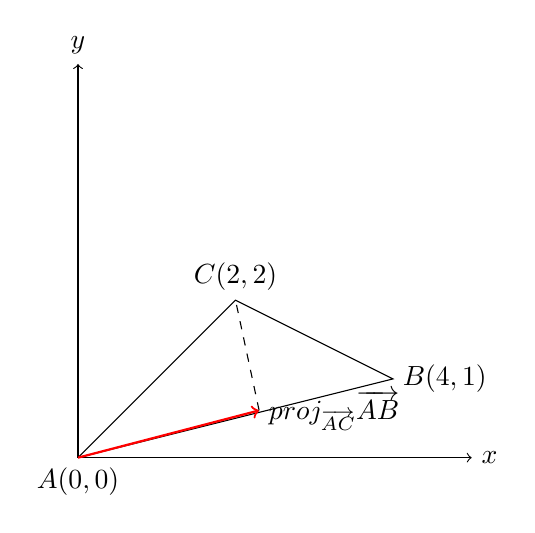
\begin{tikzpicture}
    \node[below] (A) at (0,0) {\( A(0,0) \)};
    \node[right] (B) at (4,1) {\( B(4,1) \)};
    \node[above] (C) at (2,2) {\( C(2,2) \)};
    \draw[->] (0,0)--(5,0) node[right] {\( x \)};
    \draw[->] (0,0)--(0,5) node[above] {\( y \)};
    \draw (0,0)--(4,1)--(2,2)--(0,0);
    \node[right] (D) at (2.3,0.6)
      {\( proj_{\overrightarrow{AC}}\overrightarrow{AB} \)};
    \draw[->,red,thick] (0,0)--(2.3,0.6);
    \draw[dashed] (2.3,0.6)--(2,2);
  \end{tikzpicture}
\end{center}
\begin{align*}
  comp_{\overrightarrow{AC}}\overrightarrow{AB} &=
    \frac{\overrightarrow{AB}\cdot\overrightarrow{AC}}{|\overrightarrow{AC}|} \\
  &= \frac{\langle2,2\rangle\cdot\langle4,1\rangle}{\sqrt{17}} \\
  &= \frac{10}{\sqrt{17}}
\end{align*}

\subsection*{Cross Product}
\begin{align*}
  \vec{a}\times\vec{b} &= \langle a_{2}b_{3}-a_{3}b_{2},a_{3}b_{1}-a_{1}b_{3},
  a_{1}b_{2}-a_{2}b_{1}\rangle \\
  &= \begin{bmatrix}
    \vec{i} & \vec{j} & \vec{k} \\
    a_{1} & a_{2} & a_{3} \\
    b_{1} & b_{2} & b_{3}
  \end{bmatrix} \\
  &= i\begin{bmatrix}
    a_{2} & a_{3} \\
    b_{2} & b_{3}
  \end{bmatrix}-j\begin{bmatrix}
    a_{1} & a_{3} \\
    b_{1} & b_{3}
  \end{bmatrix}-k\begin{bmatrix}
    a_{1} & a_{2} \\
    b_{1} & b_{2}
  \end{bmatrix}
\end{align*}
Properties:
\[ |\vec{a}\times\vec{b}| = |\vec{a}||\vec{b}|\sin\theta \]
The magnitude of the cross product of \( \vec{a} \) and \( \vec{b} \) is the
area of a parallelogram with sides \( \vec{a} \) and \( \vec{b} \). Since we
know this, the area of a triangle ABC is
\( \frac{1}{2}|\vec{AB}\times\vec{AC}| \).
\[ \vec{a}\times\vec{b} = \vec{0} \iff \vec{a}\parallel\vec{b} \]
If \( (\vec{a}\times\vec{b})\cdot\vec{a} = 0 \), then \( \vec{a}\times\vec{b} \)
is perpendicular to the plane described by \( \vec{a} \) and \( \vec{b} \).
\[ (\vec{a}\times\vec{b})\cdot\vec{a} =
  0 \to \vec{a}\times\vec{b}\ \bot\ \vec{a} \]
Vice versa:
\[ (\vec{a}\times\vec{b})\cdot\vec{b} =
  0 \to \vec{a}\times\vec{b}\ \bot\ \vec{b} \]
Additionally:
\begin{align*}
  \vec{a}\times\vec{b} &= -(\vec{b}\times\vec{a}) \\
  \vec{a}\times(\vec{b}+\vec{c}) &= \vec{a}\times\vec{b}+\vec{a}+\vec{c} \\
  (\lambda\vec{a})\times\vec{b} &= \lambda(\vec{a}\times\vec{b})
\end{align*}

\subsubsection*{Example}
Given a parallelopiped described by the vectors \( \vec{a},\vec{b},\vec{c} \):
\begin{align*}
V &= \text{area of base times height} \\
  &= |\vec{a}\times\vec{b}|h \\
  &= |\vec{a}\times\vec{b}|c|\cos\angle(\vec{c},\vec{a}\times\vec{b}) \\
  &= (\vec{a}\times\vec{b})\cdot\vec{c} \\
  &= \begin{vmatrix}
  c_{x} & c_{y} & c_{z} \\
  a_{x} & a_{y} & a_{z} \\
  b_{x} & b_{y} & b_{z} \\
  \end{vmatrix}
\end{align*}
Consider the following four points: A(1,1,1), B(2,1,3), C(1,2,4), D(2,2,1). Are
they coplanar? We can check if \( \vec{AB}\times\vec{AC}\parallel
\vec{DC}\times\vec{DB} \), or we can check if the volume of the parallelopiped
described by \( \vec{AB},\vec{AC},\vec{AD} \) is 0.
\[ \begin{vmatrix}
  1 & 0 & 2 \\
  0 & 1 & 3 \\
  1 & 1 & 0 \\
\end{vmatrix} = -1(-3)+0(-3)+2(-1) = -5 \ne 0 \]

\begin{center}
  If you have any questions, comments, or concerns, please contact me at
  alvin@omgimanerd.tech
\end{center}

\end{document}
